\documentclass[12pt,a4paper]{article}
\usepackage{ctex}
\usepackage{graphicx}
\usepackage{geometry}
\usepackage{array}
\usepackage{setspace}
\usepackage{xeCJK}
\usepackage{indentfirst}
\usepackage{amsmath}
\usepackage{amsthm}
\usepackage{float}
% \usepackage{subfigure}
\usepackage{booktabs}
\usepackage{multirow}
\usepackage{caption}
\usepackage{listings}
\usepackage{xcolor}
\usepackage{matlab-prettifier}
\usepackage{enumitem}
\usepackage{subcaption}
\captionsetup[table]{position=bottom}

% 页边距
\geometry{left=2.5cm,right=2.5cm,top=2.5cm,bottom=2.5cm}
% 默认宋体小四
\setCJKmainfont[BoldFont=SimHei]{SimSun}
\zihao{-4}
\linespread{1.25}

\lstdefinestyle{Matlab-boxed}{
  style=Matlab-editor,
  frame=single,
  framerule=0.6pt,
  rulecolor=\color{black},
  framesep=6pt,
  backgroundcolor=\color{black!2},
}

\begin{document}
% 实验名称（小二黑体、居中）
\begin{center}
  {\zihao{2}\heiti 稳压电路的特性与设计}
\end{center}
% 年级 专业 姓名 座位号（宋体小四、居中、段前后 0.5 行）
\vspace{0.1\baselineskip}
\begin{center}
  （\textbf{年级}\ \underline{2024 级}\quad \textbf{专业}\ \underline{x} \quad \textbf{姓名}\ \underline{Pinco Li} \quad \textbf{座位号} \ \underline{5}）
\end{center}
\vspace{0.1\baselineskip}

\section{实验目的}

\begin{enumerate}
  \item 掌握稳压电路工作原理及各元件在电路中的作用
  \item 掌握直流稳压电源的安装、调整和测试方法
  \item 熟悉和掌握线性集成稳压电路的工作原理
  \item 学习线性集成稳压电路技术指标的测量方法，包括稳压系数、纹波抑制比、输出电阻等
  \item 通过对固定输出和可调输出两种稳压电路的对比研究，理解不同电路结构对稳压性能的影响
\end{enumerate}

\section{实验仪器}

\begin{enumerate}
  \item 交流电源（输出可选 0～6 V、12 V、18 V 档位）
  \item 桥式整流电路（由 4 只 1N4007 二极管构成）
  \item 电容器（0.1 $\mu$F、1 $\mu$F、470 $\mu$F 电解电容）
  \item 三端稳压器（型号 7805）
  \item 电阻器与电位器（固定电阻若干，可调电位器 10 k$\Omega$）
  \item 双踪示波器（KEYSIGHT DSOX1202A）
  \item 数字式万用表
  \item 实验用面包板及连接导线若干
\end{enumerate}

\begin{figure}[H]
    \centering
    
\includegraphics[width=0.8\textwidth]{assets/实验装置.jpg}
    \caption{稳压电路实验装置实物图}
    \label{fig:apparatus}
\end{figure}

\section{实验原理}

\subsection{直流稳压电源的基本组成}

直流稳压电源是将交流电转换为稳定直流电的装置，其基本工作流程包括变压、整流、滤波和稳压四个环节。首先，工频交流电经过变压器降压，得到符合需要的低电压交流信号；随后，整流电路将交流信号转换为脉动的直流信号；滤波电路通过电容的充放电作用，将脉动直流中的交流成分大幅削弱，使输出波形更加平滑；最后，稳压电路进一步抑制输出电压的波动，确保在输入电压或负载电流变化时，输出电压仍能保持稳定。

\begin{figure}[H]
    \centering
    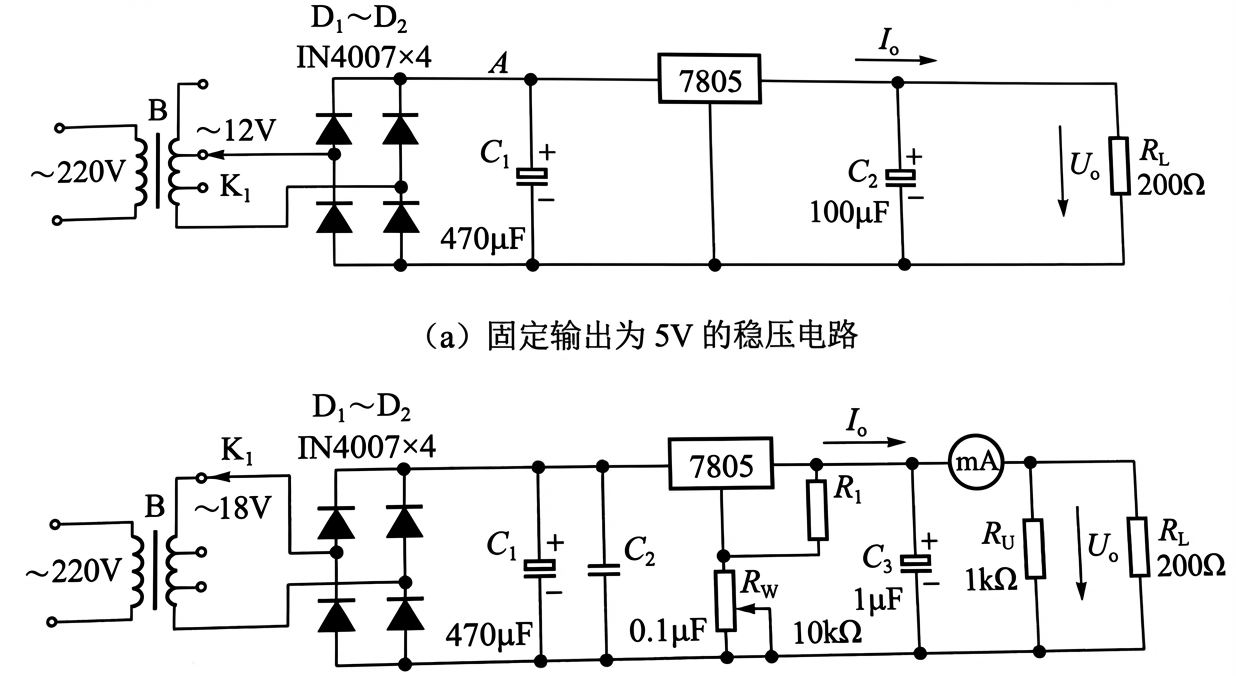
\includegraphics[width=0.5\textwidth]{assets/电路示意图.png}
    \caption{稳压电路原理示意图}
    \label{fig:circuit_diagram}
\end{figure}

在本实验中，变压器将 220 V 交流电降至 12 V，然后通过由四只二极管组成的桥式整流电路进行全波整流。桥式整流的优点在于能够充分利用变压器次级线圈的正负半周，输出的脉动直流频率是输入交流频率的两倍，有利于后续滤波。整流后的电压经过大容量电解电容滤波，将纹波电压峰峰值显著降低。最后，三端稳压器 7805 作为核心稳压元件，通过内部的基准电压源和反馈调节电路，将输出电压稳定在 5 V 左右，或者通过外接电阻实现输出电压的连续可调。

\subsection{桥式整流电路的工作原理与参数}

桥式整流电路由四只二极管按照桥式结构连接而成，其工作原理是利用二极管的单向导电性，在交流电的正半周和负半周分别使不同的二极管对导通，从而在负载上始终得到同一方向的电流。当变压器次级电压为正半周时，二极管 D1 和 D3 导通，D2 和 D4 截止；当次级电压为负半周时，D2 和 D4 导通，D1 和 D3 截止。这样，负载上得到的是频率为工频两倍的脉动直流电压。

桥式整流电路的输出平均电压与变压器次级电压有效值之间存在确定的数学关系。设变压器次级电压有效值为 $U_2$，则整流后的输出平均电压为：
\begin{align}
U_0 = \frac{1}{\pi}\int_0^{\pi} \sqrt{2} U_2 \sin\omega t \, d(\omega t) = \frac{2\sqrt{2}U_2}{\pi} \approx 0.9 U_2
\end{align}

这一关系表明，桥式整流后负载上的直流平均电压约为变压器次级电压有效值的 0.9 倍。相应地，负载电流为 $I_0 = U_0 / R_L = 0.9 U_2 / R_L$。流过每只二极管的平均电流为负载电流的一半，即 $I_{D0} = I_0 / 2$。此外，二极管承受的最大反向电压为 $U_{DRM} = \sqrt{2} U_2$，在选择二极管时必须保证其反向耐压大于此值。

\subsection{滤波电路与纹波电压}

整流后的电压虽然方向单一，但仍然是脉动的直流电压，含有大量的交流纹波成分。为了获得平滑的直流电压，需要在整流电路后加入滤波电路。最简单的滤波方式是在负载两端并联一个大容量电解电容。当整流电压升高时，电容充电，储存能量；当整流电压降低时，电容放电，向负载提供电流，从而使输出电压保持在较高的水平，减小了电压的脉动幅度。

滤波电容的容量越大、负载电阻越大（即负载电流越小），滤波效果越好，输出电压的纹波越小。纹波电压通常用峰峰值 $V_{pp}$ 来表示，它反映了输出电压中交流成分的幅度。在理想情况下，纹波电压应尽可能小，以保证负载获得纯净的直流电源。然而，仅靠电容滤波难以将纹波完全消除，因此在对输出电压稳定性要求较高的场合，还需要加入稳压电路。

\subsection{稳压电路的性能指标}

稳压电路的作用是在输入电压或负载电流发生变化时，通过内部的反馈调节机制，保持输出电压基本不变。评价稳压电路性能的主要指标包括稳压系数、纹波抑制比和输出电阻。

\paragraph{稳压系数 $S_r$}
用于衡量稳压电路对输入电压变化的抑制能力。定义为在负载电流和环境温度保持不变的条件下，输入电压相对变化量与输出电压相对变化量之比：
\begin{align}
S_r = \frac{\Delta U_o / U_o}{\Delta U_i / U_i} \bigg|_{\Delta I_O = 0, \Delta T = 0}
\end{align}

稳压系数越小，说明输入电压变化对输出电压的影响越小，稳压性能越好。理想的稳压电路应该使 $S_r$ 接近零，即无论输入电压如何变化，输出电压都保持恒定。

\paragraph{纹波抑制比 $S_{\text{inp}}$}
用于描述稳压电路对交流纹波的抑制能力，定义为输入端纹波电压峰峰值与输出端纹波电压峰峰值之比的对数值的 20 倍：

\begin{align}
S_{\text{inp}} = 20 \lg \frac{U_{\text{ipp}}}{U_{\text{opp}}} \quad (\text{单位：dB})
\end{align}

纹波抑制比的数值越大，表明稳压电路对纹波的滤除能力越强。在实际应用中，优质的稳压电源应具有较高的纹波抑制比，以保证输出电压的纯净度。

输出电阻 $R_o$ 反映了稳压电路的带负载能力，定义为在输入电压和环境温度不变的条件下，输出电压变化量与输出电流变化量之比。在实验中，可以通过测量开路输出电压 $U_o$ 和接入负载后的输出电压 $U'_o$ 来计算输出电阻：
\begin{align}
R_o = \left(\frac{U_o}{U'_o} - 1\right) \cdot R_L
\end{align}

其中 $R_L$ 为负载电阻。输出电阻越小，说明稳压电路的带负载能力越强，输出电压随负载电流变化的幅度越小。

\subsection{三端稳压器的工作原理}

三端稳压器是一种集成化的稳压器件，具有体积小、外围电路简单、性能稳定等优点，广泛应用于各种电子设备中。本实验使用的 7805 是一款正电压输出的三端稳压器，其输出电压标称值为 5 V。三端稳压器内部包含基准电压源、误差放大器、调整管和保护电路等功能模块，通过负反馈机制实现输出电压的稳定。

7805 的三个引脚分别为输入端（IN）、接地端（GND）和输出端（OUT）。当输入端电压高于输出电压约 2 V 以上时，稳压器开始正常工作。通过在输出端与接地端之间串联电阻，可以改变输出电压的大小，实现输出电压的连续可调。具体而言，输出电压为：
\begin{align}
U_o = U_{\text{ref}} \left(1 + \frac{R_2}{R_1}\right)
\end{align}

其中 $U_{\text{ref}}$ 为 7805 的基准输出电压（约 5 V），$R_1$ 为 OUT 与 GND 之间的电阻，$R_2$ 为 GND 与地之间的电阻。通过调节 $R_2$ 的大小，可以方便地调节输出电压。

\section{实验步骤}

\subsection{固定 5 V 输出稳压电路的搭建与测量}

实验开始前，首先按照电路原理图在面包板上仔细搭建固定输出为 5 V 的稳压电路。电路由工频电源、变压器、桥式整流电路、滤波电容 $C_1 = 470 \mu$F、三端稳压器 7805、输出滤波电容 $C_2 = 100 \mu$F 以及负载电阻 $R_L = 200 \Omega$ 组成。在连接电路时，需要特别注意二极管的极性方向，确保桥式整流电路连接正确，同时检查电解电容的正负极，避免接反导致电容损坏。三端稳压器 7805 的三个引脚必须按照正确的顺序连接，输入端接整流滤波后的电压，输出端接负载，接地端接电路公共地。

电路搭建完成后，将变压器的输出档位选择为 12 V，接通电源前再次仔细检查电路连接，确认无误后方可通电。使用示波器观察变压器次级输出的正弦交流信号，记录其有效值、峰峰值和频率。然后将示波器探头移至桥式整流电路的输出端，观察整流后的脉动直流信号波形，测量其有效值和平均值。接下来，测量滤波电容两端的电压波形，观察纹波电压的峰峰值，记录有效值和纹波幅度。最后，使用万用表测量稳压器输出端的直流电压，验证输出电压是否稳定在 5 V 左右。

在测量过程中，注意示波器的接地端与电路公共地必须连接在一起，避免因接地不良导致测量误差或损坏仪器。使用示波器的自动测量功能（MEASURE）可以方便地读取信号的峰峰值、有效值、平均值等参数。对于直流电压的精确测量，应使用数字万用表的直流电压档，确保量程选择合适。

\subsection{可调输出稳压电路的搭建与测量}

在完成固定输出稳压电路的测量后，进一步搭建可调输出的稳压电路。该电路在 7805 的输出端与接地端之间串联电阻 $R_1 = 100 \Omega$ 和可调电位器 $R_w$（调节范围 0～1 k$\Omega$），通过改变电位器的阻值来调节输出电压。电路中还包含滤波电容 $C_1 = 470 \mu$F、$C_2 = 0.1 \mu$F、$C_3 = 1 \mu$F，以及可调负载电阻 $R_u = 1 \text{ k}\Omega$ 和固定负载电阻 $R_L = 200 \Omega$。

电路搭建时需要特别注意的是，7805 的 GND 引脚不能直接接到电路的公共地，而是通过电阻 $R_2$ 连接到地。这样，7805 的输出电压实际上是相对于其 GND 引脚的电压，而负载两端的电压则是 7805 输出电压与 $R_2$ 上电压之和。这种接法使得输出电压可以高于 7805 的标称输出电压 5 V，实现输出电压的连续可调。

电路搭建完成后，将变压器输出档位选择为 12 V，通电后调节电位器 $R_w$，观察输出电压是否随着电位器阻值的改变而变化，以此验证电路工作是否正常。然后在 $R_w$ 的调节范围 0～600 $\Omega$ 内选取若干个阻值点（如 0、30、60、90、100、200、400、600 $\Omega$），分别测量对应的输出电压有效值和纹波电压峰峰值，记录数据并填入表格。

为了测量稳压电路的输出电阻，将电位器 $R_w$ 调至 90 $\Omega$，首先在不接负载电阻 $R_L$ 的情况下测量输出电压 $U_o$，然后接入 200 $\Omega$ 的负载电阻，再次测量输出电压 $U'_o$。根据公式 $R_o = (U_o / U'_o - 1) \cdot R_L$ 计算稳压电路的输出电阻。

\subsection{纹波抑制比的测量}

纹波抑制比是评价稳压电路滤除交流纹波能力的重要指标。在测量时，首先使用示波器测量滤波电容（稳压器输入端）两端的纹波电压峰峰值 $U_{\text{ipp}}$，这代表进入稳压器的输入纹波。然后测量稳压器输出端的纹波电压峰峰值 $U_{\text{opp}}$。根据公式 $S_{\text{inp}} = 20 \lg (U_{\text{ipp}} / U_{\text{opp}})$ 计算纹波抑制比。

在测量纹波电压时，需要将示波器的耦合方式设置为交流耦合（AC），以便滤除直流分量，更清晰地观察纹波波形。同时，适当调节示波器的垂直灵敏度和时基，使波形完整显示在屏幕上。使用示波器的峰峰值测量功能可以直接读取纹波电压的峰峰值。

\section{数据记录与处理}

\subsection{初始输入信号与滤波后信号}

\begin{figure}[H]
    \centering
    \begin{subfigure}{0.45\textwidth}
        \centering
        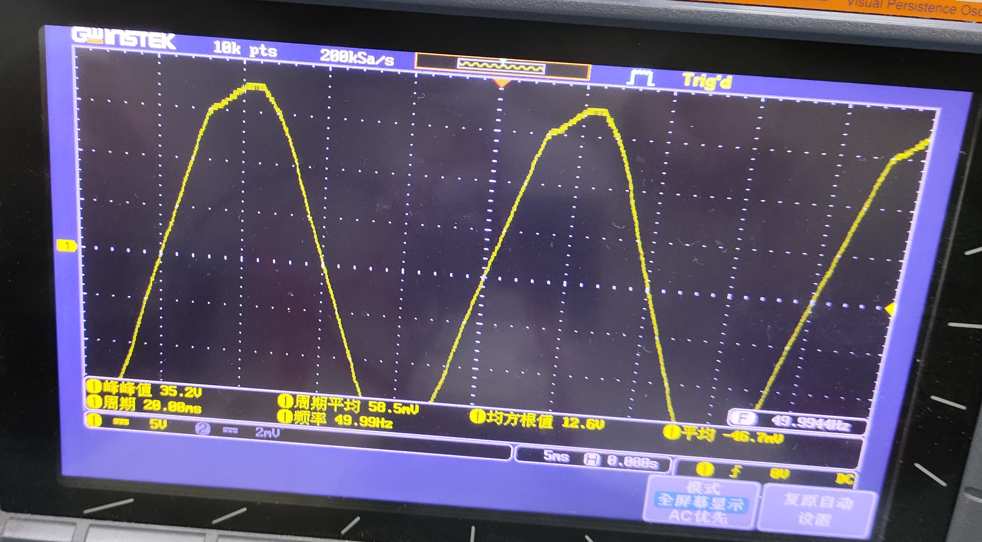
\includegraphics[width=\textwidth]{assets/初始正弦波.png}
        \caption{初始输入信号}
        \label{fig:initial_sine_wave}
    \end{subfigure}
    \hfill
    \begin{subfigure}{0.45\textwidth}
        \centering
        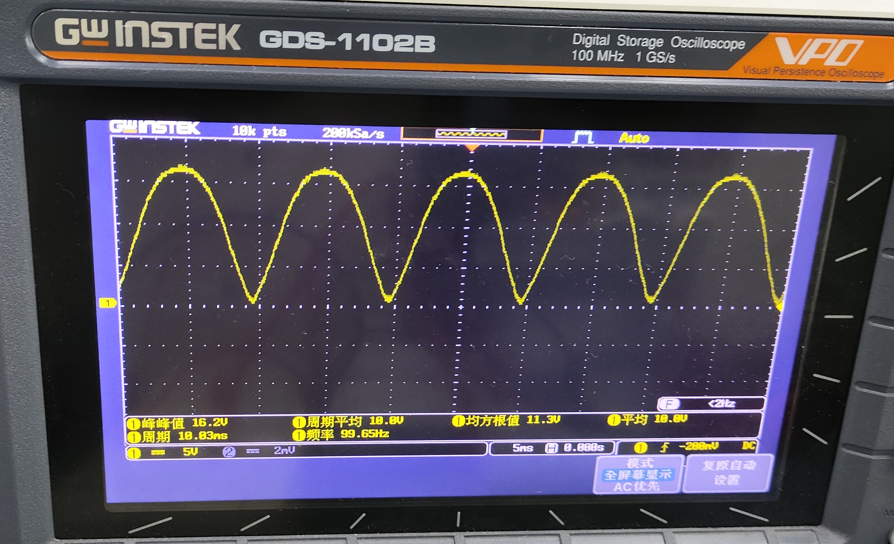
\includegraphics[width=\textwidth]{assets/整流后.png}
        \caption{整流后信号}
        \label{fig:rectified_signal}
    \end{subfigure}
    \caption{初始信号与整流后信号的对比}
    \label{fig:signal_compare}
\end{figure}


\paragraph{初始输入信号}

实验中测量了变压器次级输出的正弦交流信号以及经过桥式整流和滤波后的信号参数。变压器次级输出（12 V 档位）的有效值为 $U_0 = 12.6$ V，峰峰值为 $V_{pp} = 35.2$ V。测量值略高于变压器标称的 12 V，这是因为实际市电电压往往高于标称的 220 V。而华工变压站在向实验室供电时通常会将电压升高至略高于 220 V 的水平，以补偿输电线路的电压降，确保远端用户在负载较重时仍能获得足够的电压。因此，当输入电压高于 220 V 时，变压器次级输出电压也相应升高，本实验测得的 12.8 V 是合理的。根据正弦波的特性，峰峰值约为有效值的 $2\sqrt{2} \approx 2.83$ 倍，实测值 $35.2 / 12.6 = 2.79$，与理论值基本吻合。

\paragraph{整流后信号} 
根据桥式整流的理论，整流后的平均电压约为变压器次级电压有效值的 0.9 倍，即 $0.9 \times 12.6 = 11.34$ V，实际测得的 11.3 V，与理论值吻合。

\paragraph{整流+滤波后信号}
经过桥式整流和滤波后，在稳压器输入端测得的直流电压为 $U_0 = 14.9$ V，纹波峰峰值为 $V_{pp} = 2.60$ V（即 2600 mV）。理论上，电容滤波后，输出电压接近于输入交流电压的峰值 $\sqrt{2} \times 12.6 \approx 17.8$ V，再减去二极管压降和纹波影响，实测值 15.0 V 是合理的。

\begin{figure}[H]
    \centering
    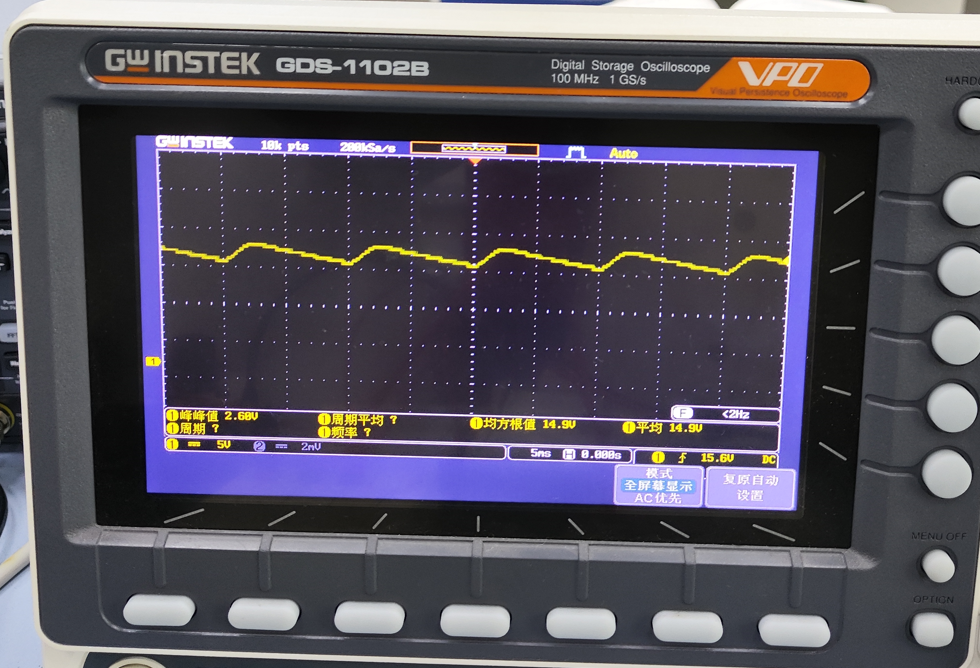
\includegraphics[width=0.5\textwidth]{assets/滤波整流后.png}
    \caption{整流+滤波后信号}
    \label{fig:filtered_rectified_signal}
\end{figure}

\paragraph{稳压后输出信号}
经过三端稳压器 7805 稳压处理后，最终输出的直流电压为 $U_0 = 5.04$ V，纹波峰峰值降至 $V_{pp} = 40.0$ mV。从示波器波形可以看出，稳压后的输出信号呈现一条非常平稳的水平线，几乎看不到明显的波动，表明稳压电路有效地抑制了输入端的纹波干扰。

输出电压为 5.04 V 而非理论值 5.00 V，这是因为三端稳压器 7805 的实际输出电压存在一定的制造容差。根据器件规格书，7805 的输出电压范围通常在 4.8～5.2 V 之间，实测值 5.04 V 在正常范围内，属于合理的器件个体差异。此外，输出端的负载电流、环境温度以及稳压器内部基准电压源的精度都会对输出电压产生微小影响。

纹波电压从稳压前的 2600 mV 大幅降低至 40 mV，纹波抑制比达到 $20 \lg (2600/40) \approx 36.26$ dB，充分体现了稳压器优异的纹波滤除能力。

\begin{figure}[H]
    \centering
    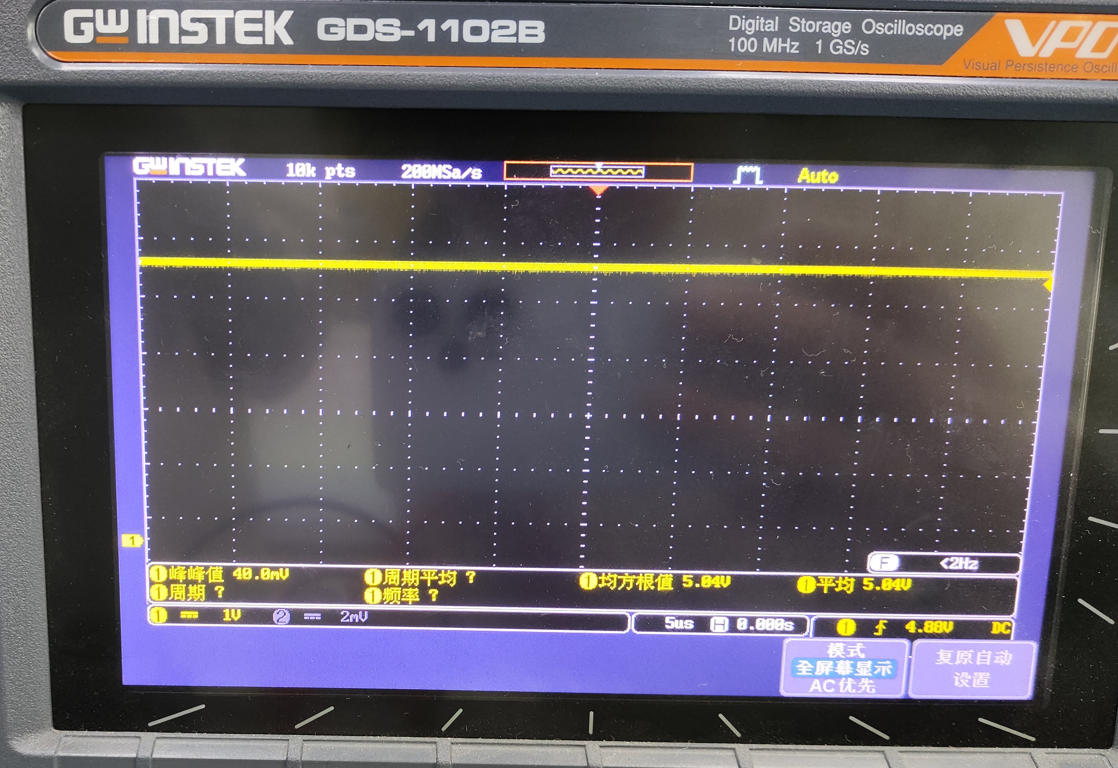
\includegraphics[width=0.5\textwidth]{assets/稳态电压.png}
    \caption{稳压后输出信号（固定5V输出）}
    \label{fig:regulated_output}
\end{figure}

\subsection{可调输出稳压电路测量数据}

在可调输出稳压电路的实验中，固定电阻 $R_1 = 100 \Omega$，可调负载电阻 $R_u = 1 \text{ k}\Omega$。通过改变调节电位器 $R_w$ 的阻值，测量不同条件下的输出电压和纹波峰峰值，实验数据如表 1 所示。

\begin{table}[H]
\centering
\begin{tabular}{|c|c|c|c|c|c|c|c|c|}
\hline
$R_w$ ($\Omega$) & 0 & 30 & 60 & 90 & 100 & 200 & 400 & 600 \\
\hline
$U_o$ (V) & 5.04 & 6.64 & 8.27 & 9.85 & 10.3 & 13.4 & 13.8 & 14.0 \\
\hline
$V_{pp}$ (mV) & 40.0 & 80.0 & 80.0 & 80.0 & 160 & 2320 & 1840 & 1440 \\
\hline
\end{tabular}
\caption{可调输出稳压电路测量数据}
\end{table}

从实验数据可以看出，随着调节电阻 $R_w$ 的增大，输出电压 $U_o$ 单调递增，这符合可调输出稳压电路的工作原理。在 $R_w$ 较小时（0～90 $\Omega$），输出电压从 5.04 V 增加到 9.85 V，纹波电压保持在较低水平（40～80 mV），说明稳压器工作在正常稳压区，具有良好的纹波抑制能力。当 $R_w$ 进一步增大（100～600 $\Omega$），输出电压继续上升至 10.3～14.0 V，但纹波电压显著增大（160～2320 mV），这表明稳压器可能已经接近或超出其正常工作范围，输入输出压差不足，导致稳压性能下降。

\subsection{输出电阻的计算}

在 $R_w = 90 \Omega$ 的条件下，测量稳压电路的输出电阻。不接负载电阻时，输出电压为 $U_o = 9.87$ V；接入 $R_L = 200 \Omega$ 负载后，输出电压为 $U'_o = 9.86$ V。根据输出电阻的计算公式：
\begin{align}
R_o = \left(\frac{U_o}{U'_o} - 1\right) \cdot R_L = \left(\frac{9.87}{9.86} - 1\right) \times 200 = 0.203 \, \Omega
\end{align}

计算结果表明，该稳压电路的输出电阻约为 0.203 $\Omega$，这是一个非常小的数值，说明稳压电路具有很强的带负载能力。当负载电流发生变化时，输出电压的变化幅度很小，能够有效维持输出电压的稳定。

\subsection{纹波抑制比的计算}

选取 $R_w = 90 \Omega$ 时的数据计算纹波抑制比。此时，稳压器输入端（滤波后）的纹波峰峰值为 $U_{\text{ipp}} = 2600$ mV，输出端的纹波峰峰值为 $U_{\text{opp}} = 80.0$ mV。根据纹波抑制比的定义：
\begin{align}
S_{\text{inp}} = 20 \lg \frac{U_{\text{ipp}}}{U_{\text{opp}}} = 20 \lg \frac{2600}{80.0} = 20 \lg 32.5 \approx 30.24 \, \text{dB}
\end{align}

纹波抑制比达到 30.24 dB，说明稳压电路将输入端的纹波电压衰减了约 32.5 倍，具有较好的纹波滤除能力。这一结果验证了稳压电路的有效性，表明三端稳压器 7805 在正常工作范围内能够显著抑制纹波干扰。

\subsection{不同 $R_w$ 下的纹波抑制比分析}

为了更全面地评估稳压电路在不同工作条件下的性能，我们计算了各个 $R_w$ 取值下的纹波抑制比，结果如表 2 所示。

\begin{table}[H]
\centering
\begin{tabular}{|c|c|c|c|}
\hline
$R_w$ ($\Omega$) & $U_o$ (V) & $V_{pp}$ (mV) & $S_{\text{inp}}$ (dB) \\
\hline
0 & 5.04 & 40.0 & 36.26 \\
\hline
30 & 6.64 & 80.0 & 30.24 \\
\hline
60 & 8.27 & 80.0 & 30.24 \\
\hline
90 & 9.85 & 80.0 & 30.24 \\
\hline
100 & 10.3 & 160 & 24.22 \\
\hline
200 & 13.4 & 2320 & 0.99 \\
\hline
400 & 13.8 & 1840 & 3.00 \\
\hline
600 & 14.0 & 1440 & 5.13 \\
\hline
\end{tabular}
\caption{不同 $R_w$ 下的纹波抑制比}
\end{table}

从表 2 可以看出，当 $R_w$ 在 0～90 $\Omega$ 范围内时，纹波抑制比保持在 30～36 dB 的较高水平，说明稳压器工作状态良好。当 $R_w = 0 \Omega$ 时，输出电压为 5.04 V，接近 7805 的标称输出电压，此时纹波抑制比最高，达到 36.26 dB。随着 $R_w$ 增大到 100 $\Omega$ 及以上，纹波抑制比急剧下降，在 $R_w = 200 \Omega$ 时仅为 0.99 dB，几乎失去了纹波抑制能力。这是因为当输出电压过高时，稳压器输入输出之间的压差减小，调整管可能工作在非线性区或接近饱和区，导致稳压性能显著恶化。

\subsection{数据处理图像分析}

图 1 展示了输出电压 $U_o$ 与调节电阻 $R_w$ 的关系曲线。从图中可以清晰地看到，输出电压随 $R_w$ 的增大而单调上升，在 $R_w$ 较小时上升速度较快，当 $R_w$ 超过 200 $\Omega$ 后，输出电压趋于平缓，最终稳定在 14.0 V 左右。这一趋势符合可调输出稳压电路的工作特性，表明通过调节电位器可以有效地改变输出电压。

\begin{figure}[H]
    \centering
    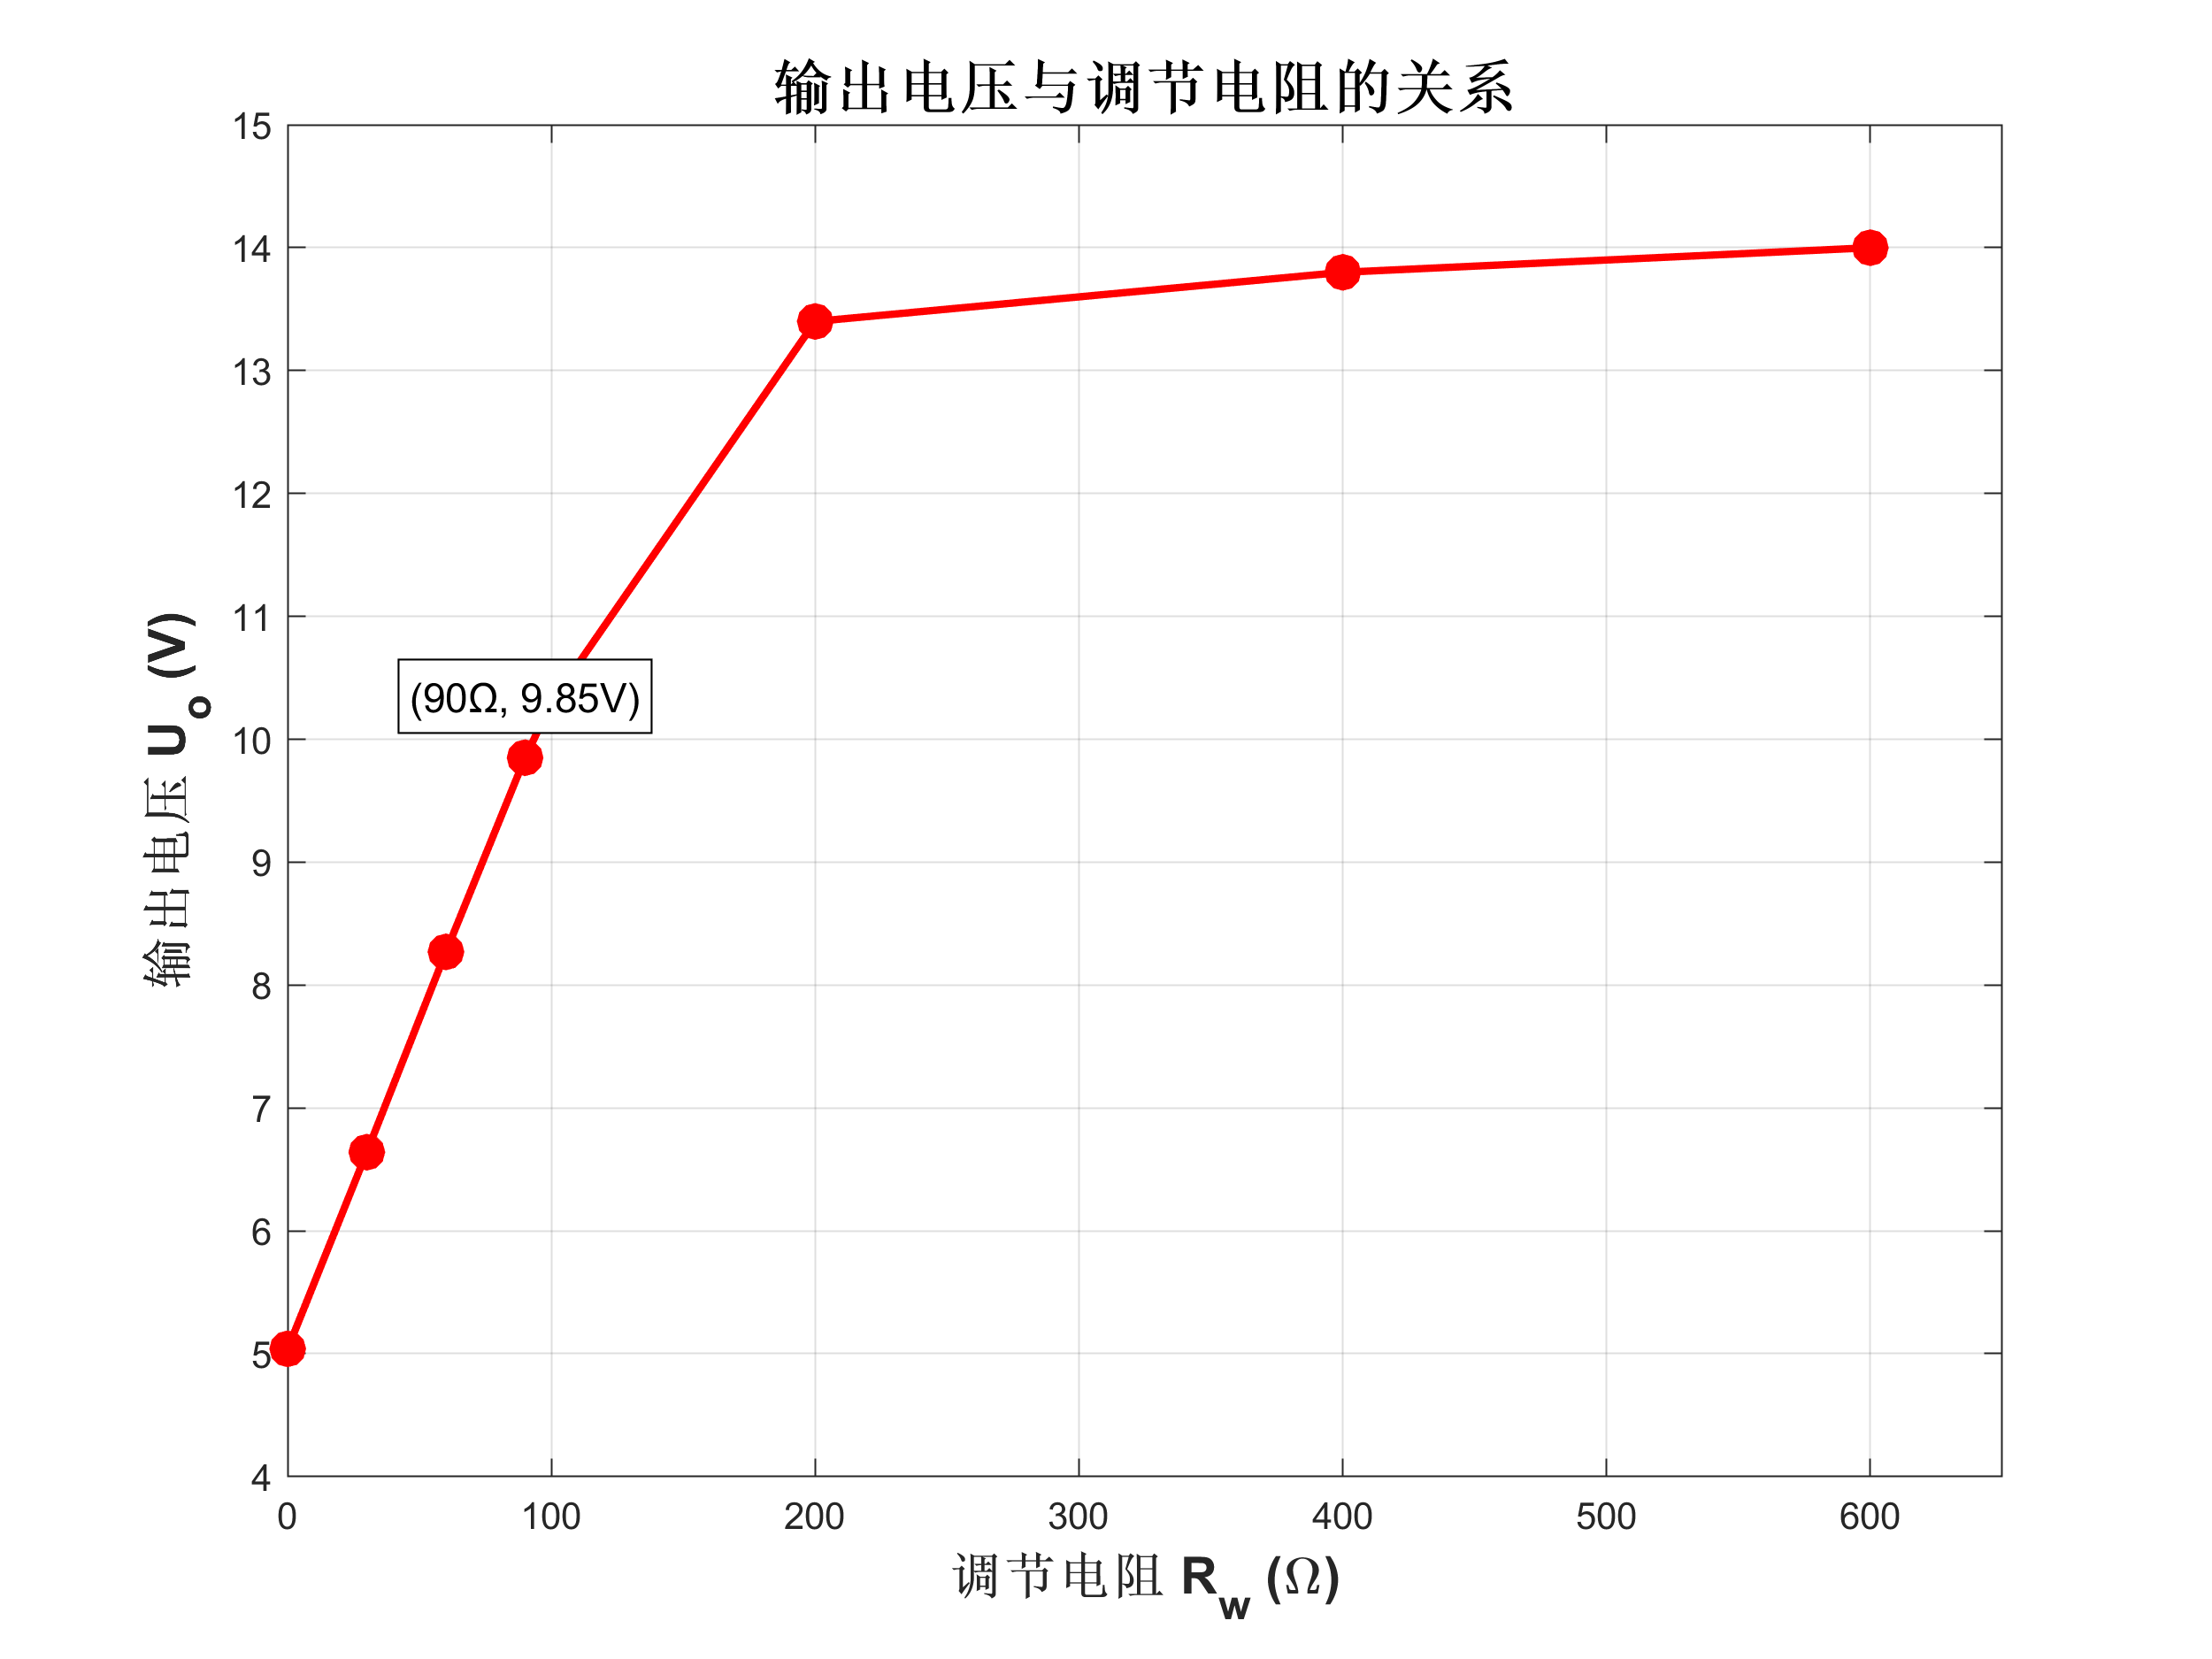
\includegraphics[width=0.75\textwidth]{assets/fig_uo_rw.png}
    \caption{输出电压与调节电阻的关系}
    \label{fig:uo_rw}
\end{figure}

图 2 采用对数坐标展示了输出纹波峰峰值 $V_{pp}$ 与调节电阻 $R_w$ 的关系。在 $R_w \leq 90 \Omega$ 时，纹波电压保持在 40～80 mV 的低水平；当 $R_w$ 增大到 100 $\Omega$ 以上时，纹波电压急剧上升，在 $R_w = 200 \Omega$ 时达到最大值 2320 mV，随后略有下降。这一现象表明，稳压电路存在一个最佳工作区域，在此区域内能够有效抑制纹波；超出此区域后，稳压性能迅速恶化。

\begin{figure}[H]
    \centering
    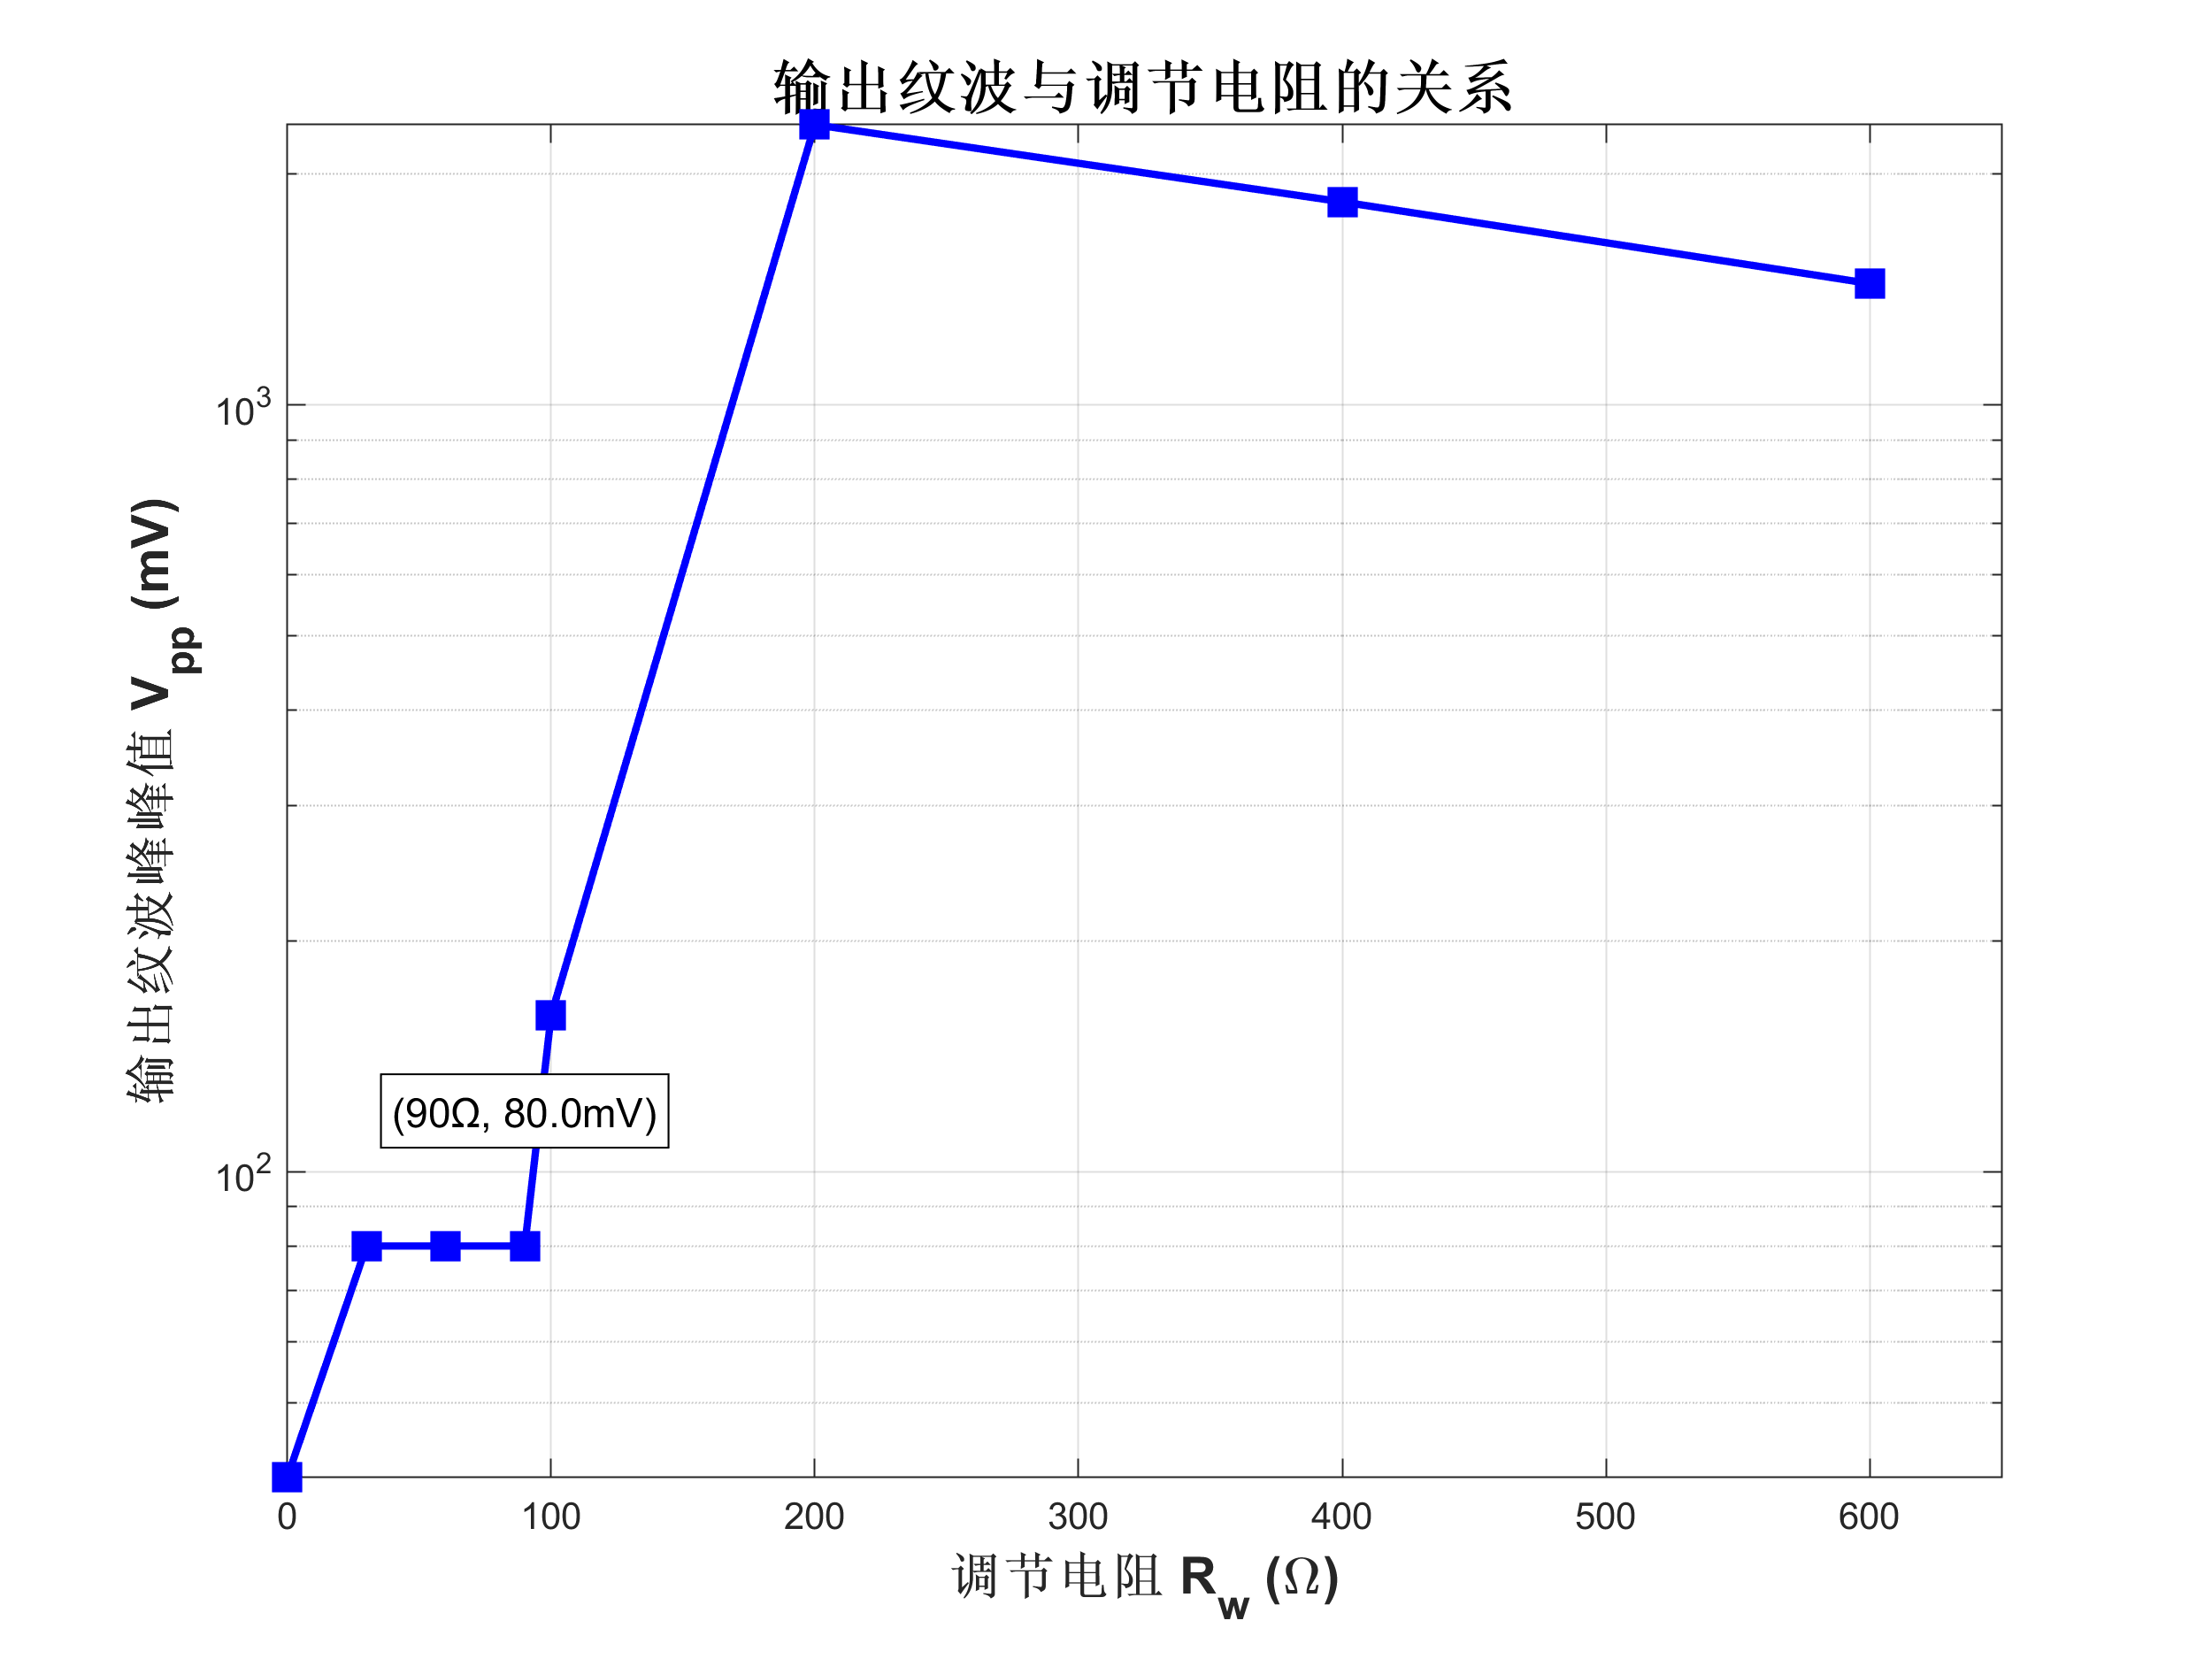
\includegraphics[width=0.75\textwidth]{assets/fig_vpp_rw.png}
    \caption{输出纹波峰峰值与调节电阻的关系}
    \label{fig:vpp_rw}
\end{figure}

综合图 1 和图 2 的分析，可以得出结论：在实际应用中，应根据负载对输出电压和纹波的要求，合理选择调节电阻的阻值。对于需要高稳定性、低纹波的应用场合，应将输出电压控制在 10 V 以下，对应的调节电阻不超过 90 $\Omega$；若需要更高的输出电压，则应考虑采用输出电压更高的稳压器，或者采用多级稳压方案。

\section{误差分析}

本实验中的测量误差主要来源于仪器精度、电路参数偏差以及实验操作等多个方面。首先，数字万用表和示波器自身存在一定的测量误差，尽管现代数字仪器的精度已经很高，但在读取电压值时仍会引入微小的系统误差。示波器在测量纹波峰峰值时，由于波形可能存在不规则的毛刺或噪声，自动测量功能的读数可能存在一定的波动，需要多次测量取平均值以提高准确性。

其次，电路元件的参数存在制造公差。电阻的标称值与实际值之间存在一定的偏差，通常为 5\% 或 1\%，这会直接影响输出电压的计算值。电解电容的容量也存在较大的容差（通常为 $\pm 20\%$），且电容的等效串联电阻（ESR）会影响滤波效果。三端稳压器 7805 的输出电压虽然标称为 5 V，但实际输出电压可能在 4.8～5.2 V 之间，这种器件间的个体差异也会带来误差。

再者，实验过程中环境温度的变化会影响元件的特性。电阻的阻值随温度有一定的温度系数，稳压器的基准电压也会受温度影响。虽然实验室温度相对稳定，但长时间通电后，电路板上的元件会发热，局部温度升高可能导致参数漂移。

实验操作方面，面包板的接触电阻不可忽略，尤其是在大电流通路中，接触不良会引起额外的电压降。连接导线的长度和布线方式也会引入寄生电感和电阻，在高频信号下可能产生影响。此外，示波器探头的接地线过长或接地不良，会引入干扰信号，影响纹波电压的测量准确性。

在计算输出电阻时，由于输出电压变化量很小（仅 0.01 V），对测量精度要求很高。万用表的最小分辨率如果为 0.01 V，则测量的相对误差可能较大。为了提高测量精度，可以采用更高精度的数字电压表，或者增大负载变化幅度，使输出电压变化更加明显。

对于纹波抑制比的测量，输入纹波和输出纹波的峰峰值相差较大，示波器的垂直灵敏度需要进行调整，两次测量的条件不完全一致，可能引入系统误差。此外，电源本身的输出波动、市电电压的瞬时变化等外部因素也会对实验结果产生影响。

综合以上分析，本实验的主要误差来源可以归纳为仪器系统误差、元件参数误差、环境因素影响以及操作随机误差。通过多次测量取平均值、改善接触状况、使用高精度仪器、保持环境稳定等措施，可以有效减小实验误差，提高测量结果的可靠性。

\section{实验结论}

通过本次直流稳压电源实验，成功搭建了固定输出和可调输出两种类型的稳压电路，并对其主要性能参数进行了系统的测量与分析。实验结果表明，采用桥式整流、电容滤波和三端稳压器 7805 构成的稳压电路能够有效地将交流电转换为稳定的直流电，输出电压稳定，纹波抑制效果良好。

在可调输出稳压电路中，通过改变调节电阻 $R_w$ 的阻值，实现了输出电压在 5～14 V 范围内的连续可调。实验数据显示，当 $R_w$ 在 0～90 $\Omega$ 范围内时，稳压电路工作在最佳状态，输出电压稳定，纹波峰峰值保持在 40～80 mV 的低水平，纹波抑制比达到 30～36 dB。在 $R_w = 90 \Omega$ 时，输出电压为 9.85 V，输出电阻仅为 0.203 $\Omega$，表现出优异的带负载能力和稳压性能。

当 $R_w$ 增大到 100 $\Omega$ 以上时，虽然输出电压继续升高，但纹波电压急剧增大，纹波抑制比显著下降，稳压性能恶化。这是因为输出电压过高导致稳压器输入输出压差不足，调整管无法维持正常的稳压状态。这一现象提醒我们，在实际应用中必须根据稳压器的工作特性和负载要求，合理设计电路参数，确保稳压器工作在最佳区域。

实验过程中，通过使用示波器观察各测试点的波形，直观地理解了整流、滤波、稳压各环节对信号的作用。变压器次级输出的正弦波经过桥式整流后变为脉动直流，频率加倍；经过电容滤波后，波形趋于平滑，纹波幅度显著减小；最后经过稳压器输出，得到稳定的直流电压，纹波进一步被抑制。这一系列变化清晰地展现了直流稳压电源的工作过程。

此外，实验强化了对稳压电路性能指标的理解。稳压系数反映了电路对输入电压波动的抑制能力，纹波抑制比体现了对交流干扰的滤除效果，输出电阻则表征了带负载的能力。这些参数从不同角度全面评价了稳压电源的性能，为实际应用中选择和设计稳压电路提供了重要依据。

通过本次实验，不仅掌握了直流稳压电源的基本原理和设计方法，还锻炼了电路搭建、仪器使用、数据处理和结果分析等实验技能。实验中遇到的问题，如接线错误、波形不稳定、测量数据异常等，通过仔细检查和分析，均得到了妥善解决，积累了宝贵的实践经验。这些知识和技能将为今后的电子技术学习和工程实践奠定坚实的基础。

\clearpage
\appendix

\section{数据处理 MATLAB 代码}

\begin{lstlisting}[style=Matlab-boxed,caption={直流稳压电源数据处理代码}]
clear; clc; close all;

%% 第一组数据：改变Rw时的输出电压和纹波
Rw = [0, 30, 60, 90, 100, 200, 400, 600]; % 欧姆
Uo = [5.04, 6.64, 8.27, 9.85, 10.3, 13.4, 13.8, 14.0]; % V
Vpp = [40.0, 80.0, 80.0, 80.0, 160, 2320, 1840, 1440]; % mV

%% 第二组数据：初始输入正弦波
U_input = 12.8; % V
Vpp_input = 36.0; % V

%% 第三组数据：滤波后电压
U_filter = 15.0; % V
Vpp_filter = 2.60; % V (转换为mV: 2600 mV)

%% 第四组数据：输出电阻计算
Rw_test = 90; % 欧姆
U_no_load = 9.87; % V
U_with_load = 9.86; % V
R_load = 200; % 欧姆
R_output = (U_no_load / U_with_load - 1) * R_load;

fprintf('========== 计算结果 ==========\n');
fprintf('输出电阻 Ro = %.4f Omega\n\n', R_output);

%% 计算纹波抑制比（以Rw=90欧为例）
idx_90 = find(Rw == 90);
Vpp_output_90 = Vpp(idx_90); % mV
Vpp_filter_mV = 2600; % mV
Sinp = 20 * log10(Vpp_filter_mV / Vpp_output_90);
fprintf('纹波抑制比 (Rw=90Omega): Sinp = %.2f dB\n', Sinp);
fprintf('输入纹波 Vpp = %.2f mV\n', Vpp_filter_mV);
fprintf('输出纹波 Vpp = %.2f mV\n\n', Vpp_output_90);

%% 绘图1：输出电压与Rw的关系
figure('Color','w', 'Position', [100, 100, 800, 600]);
plot(Rw, Uo, 'ro-', 'MarkerSize', 8, 'MarkerFaceColor', 'r', 'LineWidth', 2);
grid on;
xlabel('调节电阻 R_w (\Omega)', 'FontSize', 14, 'FontWeight', 'bold');
ylabel('输出电压 U_o (V)', 'FontSize', 14, 'FontWeight', 'bold');
title('输出电压与调节电阻的关系', 'FontSize', 16, 'FontWeight', 'bold');
xlim([0, 650]);
ylim([4, 15]);

% 标注关键点
text(90, 9.85+0.5, sprintf('(90\Omega, %.2fV)', 9.85), 'FontSize', 11, ...
    'HorizontalAlignment', 'center', 'BackgroundColor', 'w', 'EdgeColor', 'k');

%% 绘图2：输出纹波与Rw的关系
figure('Color','w', 'Position', [150, 150, 800, 600]);
semilogy(Rw, Vpp, 'bs-', 'MarkerSize', 8, 'MarkerFaceColor', 'b', 'LineWidth', 2);
grid on;
xlabel('调节电阻 R_w (\Omega)', 'FontSize', 14, 'FontWeight', 'bold');
ylabel('输出纹波峰峰值 V_{pp} (mV)', 'FontSize', 14, 'FontWeight', 'bold');
title('输出纹波与调节电阻的关系', 'FontSize', 16, 'FontWeight', 'bold');
xlim([0, 650]);

% 标注关键点
text(90, 80*1.5, sprintf('(90\Omega, %.1fmV)', 80.0), 'FontSize', 11, ...
    'HorizontalAlignment', 'center', 'BackgroundColor', 'w', 'EdgeColor', 'k');

%% 计算不同Rw下的纹波抑制比
fprintf('不同Rw下的纹波抑制比：\n');
fprintf('Rw(\Omega)\tUo(V)\tVpp(mV)\tSinp(dB)\n');
fprintf('----------------------------------------\n');
for i = 1:length(Rw)
    Sinp_i = 20 * log10(Vpp_filter_mV / Vpp(i));
    fprintf('%d\t%.2f\t%.1f\t%.2f\n', Rw(i), Uo(i), Vpp(i), Sinp_i);
end

%% 保存图片
print(gcf, 'assets/fig_vpp_rw.png', '-dpng', '-r300');
figure(1);
print(gcf, 'assets/fig_uo_rw.png', '-dpng', '-r300');

fprintf('\n图片已保存到 assets/ 目录\n');
\end{lstlisting}

\end{document}

